\documentclass{../lista}

\begin{document}
	\cabecalho{1}{Questões}{Terra, Lua e Sol}{Iago Mendes}

	\begin{questao}{1 ponto}
		Os primeiros eclipses foram registados há cerca de 4 mil anos na Babilônia. Ao longo da história, eles provocaram medo e admiração. Ao observarem os eclipses, povos de diferentes épocas relacionaram esse fenômeno à intervenção de figuras mitológicas que tentariam devorar os astros e a sua luz.

		\begin{pergunta}{0,5 ponto}
			Analise as 2 astrofotos abaixo -- tiradas pelo autor desta lista :) -- e marque o item que mostra um eclipse.
			\begin{multicols}{2}
				\begin{figure}[H]
					\centering
					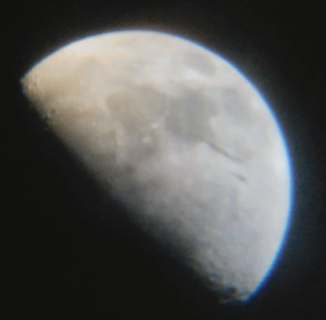
\includegraphics[height=.75\linewidth]{./img/1a.png}
					\captionsetup{labelformat=empty}
					\caption{(a)}
				\end{figure}
				\begin{figure}[H]
					\centering
					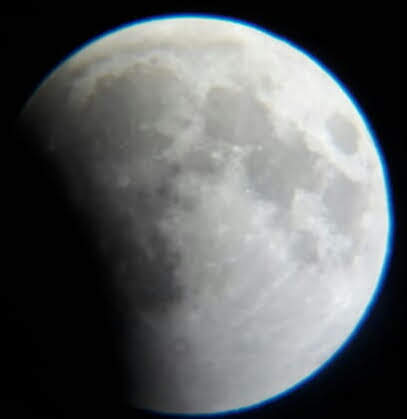
\includegraphics[height=.75\linewidth]{./img/1b.jpg}
					\captionsetup{labelformat=empty}
					\caption{(b)}
				\end{figure}
			\end{multicols}
		\end{pergunta}

		\begin{pergunta}{0.25 ponto}
			Que tipo de eclipse é mostrado?
			\begin{alternativas}
				\item Eclipse lunar
				\item Eclipse solar
			\end{alternativas}
		\end{pergunta}
		
		\begin{pergunta}{0.25 ponto}
			Em qual fase lunar esse eclipse aconteceu?
			\begin{alternativas}
				\item Lua Nova
				\item Lua Crescente
				\item Lua Cheia
				\item Lua Minguante
			\end{alternativas}
		\end{pergunta}
	\end{questao}

	\begin{questao}{1 ponto}
		Analise, mais uma vez, a imagem do item que você \textbf{não} marcou como sendo um eclipse na questão anterior. Ela foi tirada no Hemisfério Sul por meio de um telescópio refletor. A imagem está exatamente como é observada na lente ocular, a qual produz uma imagem invertida.
		\begin{pergunta}{1 ponto}
			Levando em consideração o que foi dito, em qual fase lunar essa foto foi tirada?
			\begin{alternativas}
				\item Lua Nova
				\item Lua Crescente
				\item Lua Cheia
				\item Lua Minguante
			\end{alternativas}
		\end{pergunta}
	\end{questao}

	\begin{questao}{1 ponto}
		1 ano terrestre é comumente relacionado ao intervalo de tempo correspondente à translação completa da Terra em torno do Sol. Contudo, o valor exato de 1 ano varia de acordo com o método de análise. Nesse sentido, temos duas definições principais para essa medida de tempo: Ano Tropical e Ano Sideral.
		\begin{pergunta}{0,25 ponto}
			Qual o referencial na medida do Ano Tropical?
			\begin{alternativas}
				\item Movimento Retrógrado de Marte
				\item Equinócio Vernal (início das estações do ano)
				\item Ápex (ponto para o qual o Sol se dirige)
				\item Periélio ou Afélio
			\end{alternativas}
		\end{pergunta}
		\begin{pergunta}{0,25 ponto}
			Qual o referencial na medida do Ano Sideral?
			\begin{alternativas}
				\item Planetas do Sistema Solar
				\item Galáxia de Andrômeda
				\item Quasares
				\item Estrelas de Fundo
			\end{alternativas}
		\end{pergunta}
		\begin{pergunta}{0,25 ponto}
			O Ano Tropical tem duração de 365,2564 dias solares médios, enquanto o Ano Sideral possui 365,2422 dias solares médios. Qual é o \textbf{principal} movimento terrestre responsável por essa diferença?
			\begin{alternativas}
				\item Rotação da Terra
				\item Translação da Terra
				\item Precessão dos Equinócios
				\item Nutação
			\end{alternativas}
		\end{pergunta}
		\begin{pergunta}{0,25 ponto}
			Geralmente, usamos 365,25 dias solares médios como uma aproximação para a duração do ano na Astronomia. Contudo, o nosso calendário possui 365 dias, o que deixa cerca de $\frac{1}{4}$ dia sobrando. Para consertar isso, temos o ano bissexto, o qual possui 366 dias solares médios e segue uma regra de 3 exigências. Pensando nisso, marque a seguir somente o(s) ano(s) que é(são) bissexto(s):
			\begin{alternativas}
				\item 2400
				\item 1846
				\item 2100
				\item 1960
			\end{alternativas}
		\end{pergunta}
	\end{questao}

	\begin{questao}{1 ponto}
		Loinha -- uma estudante que usou muito o site da LOA -- foi medalhista de ouro na OBA e está atualmente estudando para as Seletivas. Em seus estudos, deparou-se com vários esquemas altazimutais e resolveu criar um com base no seu local de moradia. Assim, ela desenhou a seguinte representação:
		\begin{figure}[H]
			\centering
			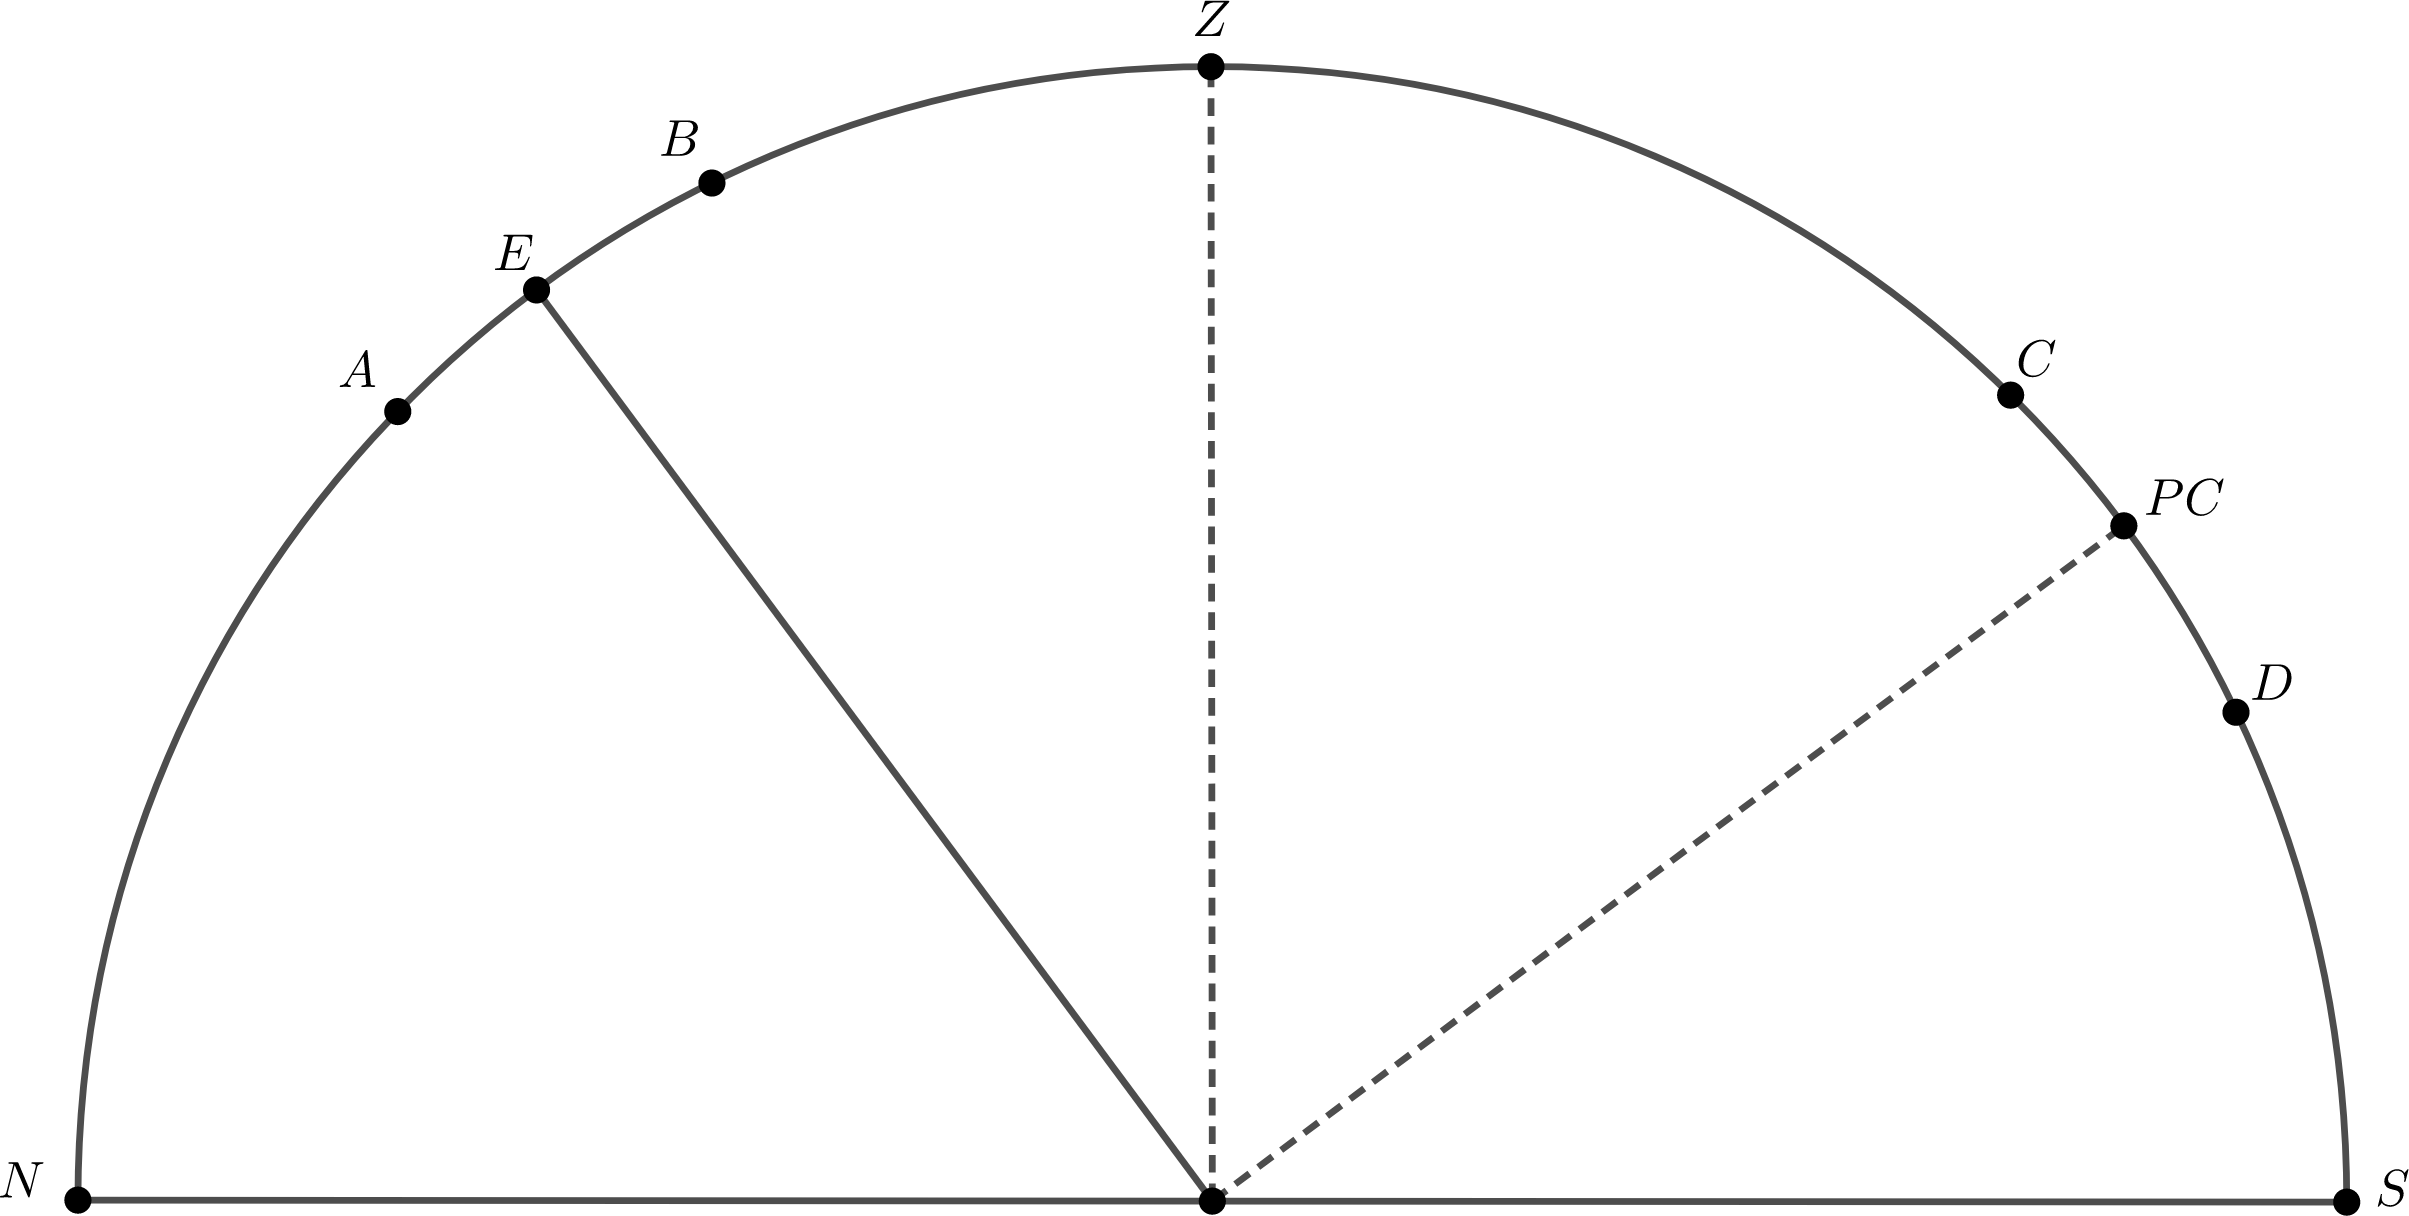
\includegraphics[scale=1.2]{./img/4.png}
		\end{figure}
		Nela, a linha horizontal representa o horizonte; o semiarco, a esfera celeste; $N$ e $S$, pontos cardeais norte e sul, respectivamente; $E$, o equador celeste (perceba que estamos olhando de lado, o que torna uma circunferência num segmento de reta); $PC$, o Polo Celeste elevado; $Z$, o zênite; e $A$, $B$, $C$ e $D$ pontos estratégicos na esfera celeste. \linebreak
		Como Loinha adora colocar em prática os conceitos aprendidos no site da LOA, fez alguns registros. Primeiramente, anotou a data e o horário: 22/06 (solstício de junho) ao meio-dia.\linebreak
		Observação: considere o mesmo horário para as perguntas.
			\begin{pergunta}{0,5 ponto}
				Depois, ele decidiu registrar em que posição o Sol se encontrava naquele momento. Qual a resposta correta?
				\begin{alternativas}
					\item $A$
					\item $B$
					\item $C$
					\item $D$
				\end{alternativas}
			\end{pergunta}

			\begin{pergunta}{0,5 ponto}
				Animado para ver o comportamento das sombras, Loinha fincou uma haste na projeção do zênite no chão (centro da semicircunferência). Com a ajuda de uma bússola, anotou a direção cardeal para a qual a sombra apontava. Qual foi a anotação?
				\begin{alternativas}
					\item Norte
					\item Leste
					\item Sul
					\item Oeste
				\end{alternativas}
			\end{pergunta}
	\end{questao}

	\begin{questao}{1 ponto}
		Para as perguntas desta questão, considere o contexto da questão anterior.

		\begin{pergunta}{0,5 ponto}
			Em que lugar Loinha mora?
			\begin{alternativas}
				\item Hemisfério Norte
				\item Equador
				\item Hemisfério Sul
			\end{alternativas}
		\end{pergunta}

		\begin{pergunta}{0,5 ponto}
			No momento dos registros, que solstício estava ocorrendo no Hesisfério Norte e Sul, respectivamente?
			\begin{alternativas}
				\item Solstício de Verão e Solstício de Verão
				\item Solstício de Verão e Solstício de Inverno
				\item Solstício de Inverno e Solstício de Inverno
				\item Solstício de Inverno e Solstício de Verão
			\end{alternativas}
		\end{pergunta}
	\end{questao}

	\encerramento
\end{document}